% GNUPLOT: LaTeX picture with Postscript
\begingroup
  \makeatletter
  \providecommand\color[2][]{%
    \GenericError{(gnuplot) \space\space\space\@spaces}{%
      Package color not loaded in conjunction with
      terminal option `colourtext'%
    }{See the gnuplot documentation for explanation.%
    }{Either use 'blacktext' in gnuplot or load the package
      color.sty in LaTeX.}%
    \renewcommand\color[2][]{}%
  }%
  \providecommand\includegraphics[2][]{%
    \GenericError{(gnuplot) \space\space\space\@spaces}{%
      Package graphicx or graphics not loaded%
    }{See the gnuplot documentation for explanation.%
    }{The gnuplot epslatex terminal needs graphicx.sty or graphics.sty.}%
    \renewcommand\includegraphics[2][]{}%
  }%
  \providecommand\rotatebox[2]{#2}%
  \@ifundefined{ifGPcolor}{%
    \newif\ifGPcolor
    \GPcolortrue
  }{}%
  \@ifundefined{ifGPblacktext}{%
    \newif\ifGPblacktext
    \GPblacktexttrue
  }{}%
  % define a \g@addto@macro without @ in the name:
  \let\gplgaddtomacro\g@addto@macro
  % define empty templates for all commands taking text:
  \gdef\gplbacktext{}%
  \gdef\gplfronttext{}%
  \makeatother
  \ifGPblacktext
    % no textcolor at all
    \def\colorrgb#1{}%
    \def\colorgray#1{}%
  \else
    % gray or color?
    \ifGPcolor
      \def\colorrgb#1{\color[rgb]{#1}}%
      \def\colorgray#1{\color[gray]{#1}}%
      \expandafter\def\csname LTw\endcsname{\color{white}}%
      \expandafter\def\csname LTb\endcsname{\color{black}}%
      \expandafter\def\csname LTa\endcsname{\color{black}}%
      \expandafter\def\csname LT0\endcsname{\color[rgb]{1,0,0}}%
      \expandafter\def\csname LT1\endcsname{\color[rgb]{0,1,0}}%
      \expandafter\def\csname LT2\endcsname{\color[rgb]{0,0,1}}%
      \expandafter\def\csname LT3\endcsname{\color[rgb]{1,0,1}}%
      \expandafter\def\csname LT4\endcsname{\color[rgb]{0,1,1}}%
      \expandafter\def\csname LT5\endcsname{\color[rgb]{1,1,0}}%
      \expandafter\def\csname LT6\endcsname{\color[rgb]{0,0,0}}%
      \expandafter\def\csname LT7\endcsname{\color[rgb]{1,0.3,0}}%
      \expandafter\def\csname LT8\endcsname{\color[rgb]{0.5,0.5,0.5}}%
    \else
      % gray
      \def\colorrgb#1{\color{black}}%
      \def\colorgray#1{\color[gray]{#1}}%
      \expandafter\def\csname LTw\endcsname{\color{white}}%
      \expandafter\def\csname LTb\endcsname{\color{black}}%
      \expandafter\def\csname LTa\endcsname{\color{black}}%
      \expandafter\def\csname LT0\endcsname{\color{black}}%
      \expandafter\def\csname LT1\endcsname{\color{black}}%
      \expandafter\def\csname LT2\endcsname{\color{black}}%
      \expandafter\def\csname LT3\endcsname{\color{black}}%
      \expandafter\def\csname LT4\endcsname{\color{black}}%
      \expandafter\def\csname LT5\endcsname{\color{black}}%
      \expandafter\def\csname LT6\endcsname{\color{black}}%
      \expandafter\def\csname LT7\endcsname{\color{black}}%
      \expandafter\def\csname LT8\endcsname{\color{black}}%
    \fi
  \fi
  \setlength{\unitlength}{0.0500bp}%
  \begin{picture}(7200.00,5040.00)%
    \gplgaddtomacro\gplbacktext{%
      \csname LTb\endcsname%
      \put(1078,1364){\makebox(0,0)[r]{\strut{} 0.05}}%
      \put(1078,1790){\makebox(0,0)[r]{\strut{} 0.06}}%
      \put(1078,2217){\makebox(0,0)[r]{\strut{} 0.07}}%
      \put(1078,2643){\makebox(0,0)[r]{\strut{} 0.08}}%
      \put(1078,3070){\makebox(0,0)[r]{\strut{} 0.09}}%
      \put(1078,3496){\makebox(0,0)[r]{\strut{} 0.1}}%
      \put(1078,3922){\makebox(0,0)[r]{\strut{} 0.11}}%
      \put(1078,4349){\makebox(0,0)[r]{\strut{} 0.12}}%
      \put(1078,4775){\makebox(0,0)[r]{\strut{} 0.13}}%
      \put(1210,1144){\makebox(0,0){\strut{} 12}}%
      \put(1909,1144){\makebox(0,0){\strut{} 14}}%
      \put(2608,1144){\makebox(0,0){\strut{} 16}}%
      \put(3307,1144){\makebox(0,0){\strut{} 18}}%
      \put(4007,1144){\makebox(0,0){\strut{} 20}}%
      \put(4706,1144){\makebox(0,0){\strut{} 22}}%
      \put(5405,1144){\makebox(0,0){\strut{} 24}}%
      \put(6104,1144){\makebox(0,0){\strut{} 26}}%
      \put(6803,1144){\makebox(0,0){\strut{} 28}}%
      \put(176,3069){\rotatebox{-270}{\makebox(0,0){\strut{}$d$}}}%
      \put(4006,814){\makebox(0,0){\strut{}$\sqrt{\frac{U_\text{B}}{1\text V}}/\frac{I_\text{H}}{1\text A}$}}%
    }%
    \gplgaddtomacro\gplfronttext{%
      \csname LTb\endcsname%
      \put(2064,393){\makebox(0,0)[r]{\strut{}U$_\text{B}$=160V}}%
      \csname LTb\endcsname%
      \put(2064,173){\makebox(0,0)[r]{\strut{}U$_\text{B}$=140V}}%
      \csname LTb\endcsname%
      \put(4239,393){\makebox(0,0)[r]{\strut{}I$_\text{H}$=0.5A}}%
      \csname LTb\endcsname%
      \put(4239,173){\makebox(0,0)[r]{\strut{}$I_\text{H}$=0.7}}%
      \csname LTb\endcsname%
      \put(6414,393){\makebox(0,0)[r]{\strut{}Regression}}%
    }%
    \gplbacktext
    \put(0,0){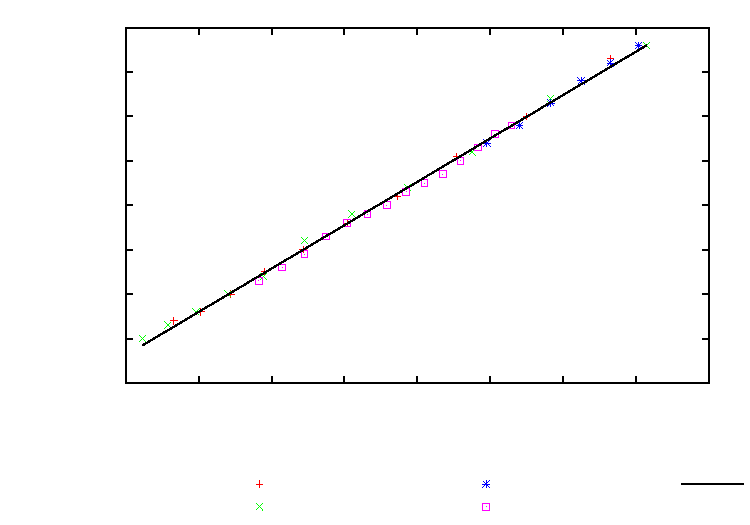
\includegraphics{UI}}%
    \gplfronttext
  \end{picture}%
\endgroup
